\dev{Emile Martinez}{}


\textit{Ce développement a pour but de décrire les critères de test, en illustrant sur l'exemple du maximum ou on illustre les erreurs. On finit par une preuve de l'indécidabilité de la satisfiabilité de ces critères de test} \\ \\
\paragraph{Tous les noeuds} On souhaite au moins vérifier chaque ligne de code 
\\
\begin{minipage}{0.5\linewidth}
	\begin{lstlisting}
max(a,b):
    int res;
    if(a < b)
        res = b;
    else
        res = a <@\textcolor{red}{+ 1}@>;
    return res
	\end{lstlisting}
\end{minipage} 
\begin{minipage}{0.5\linewidth}
	\begin{center}
		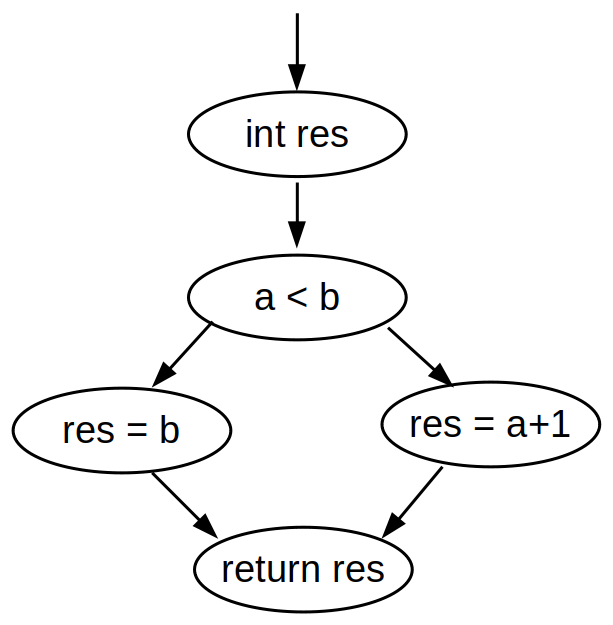
\includegraphics[scale=0.2]{Developpements/critere de test/cas_11.png}
	\end{center}
\end{minipage}

% Les flèches ne sont pas assez belles, et j'ai la flemme de perdre trop de temps avec ça
%\tikzset{elliptic state/.style={draw,ellipse}}
%\begin{tikzpicture}[->, node distance = 1.5cm]
%	\node[] (q-1) {};
%	\node[elliptic state, below of = q-1] (q0) {int res};
%	\node[elliptic state, below of = q0] (q1) {a $<$ b};
%	\node[elliptic state, below left =0.8cm and 1.3cm of q1] (q2) {res = b};
%	\node[elliptic state, below right = 0.8cm and 1.3cm of q1] (q3) {res = a + 1};
%	\node[elliptic state, below right = 0.8cm and 1.3cm of q2] (q4) {return res};
%	
%	\draw (q-1) edge[] node{} (q0) ;
%	\draw (q0) edge[] node{} (q1) ;
%	\draw (q1) edge[] node{} (q2) ;
%	\draw (q1) edge[] node{} (q3) ;
%	\draw (q2) edge[] node{} (q4) ;
%	\draw (q3) edge[] node{} (q4) ;
%	
%\end{tikzpicture}

$DT = [((3,5), 5)]$ \raisebox{-0.5\height}{	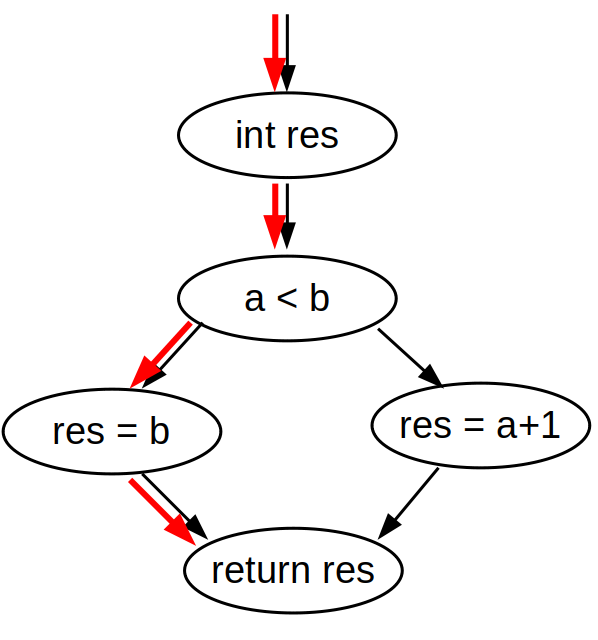
\includegraphics[scale=0.2]{Developpements/critere de test/cas_12.png}} On ne détecte pas l'erreur.\\

On cherche alors à couvrir tous les noeuds $DT = [((3,5), 5), ((5,4), 5)]$ \raisebox{-0.5\height}{	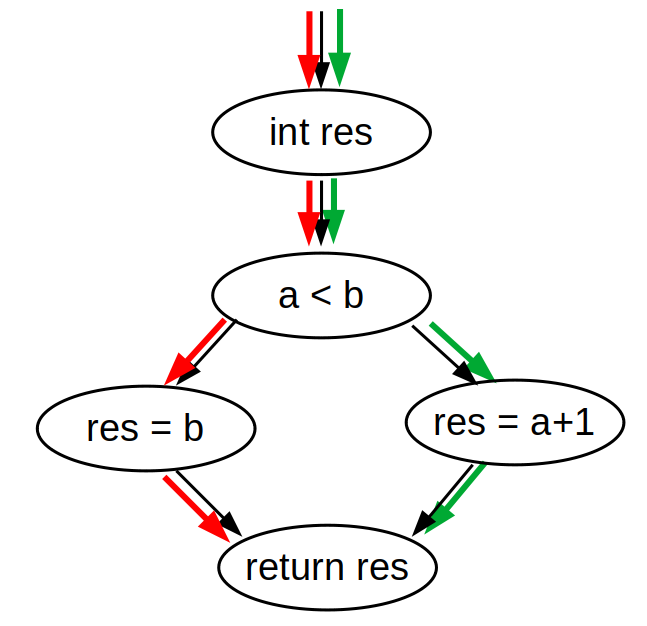
\includegraphics[scale=0.2]{Developpements/critere de test/cas_13.png}}

\paragraph{Tous les arcs} Néanmoins, ce critère n'est pas suffisant.
\\
\begin{minipage}{0.5\linewidth}
\begin{lstlisting}
max(a,b):
    int res = a <@\textcolor{red}{+1}@>;
    if (a < b)
        res = b;
    return res;
\end{lstlisting}
\end{minipage}
\begin{minipage}{0.5\linewidth}
	\begin{center}
		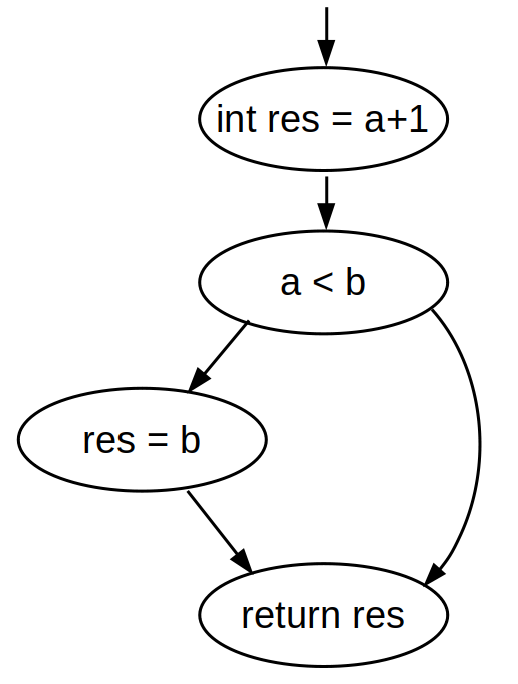
\includegraphics[scale=0.2]{Developpements/critere de test/cas_21.png}
	\end{center}
\end{minipage}

$DT = [((3,5), 5)]$ couvre tous les noeuds mais ne détecte pas l'erreur \raisebox{-0.5\height}{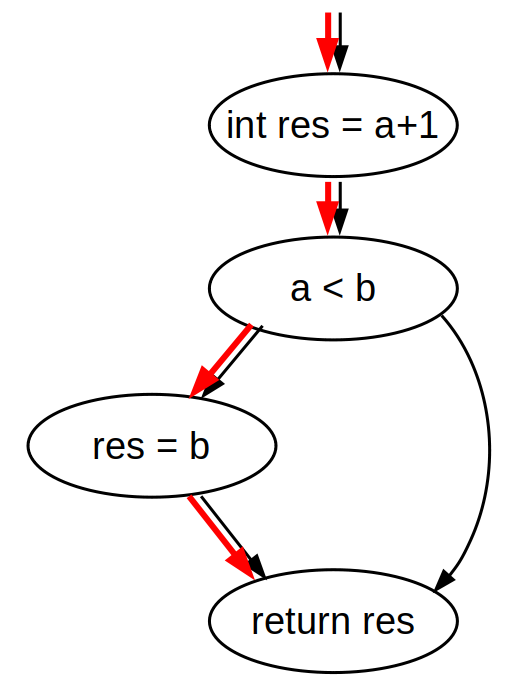
\includegraphics[scale=0.2]{Developpements/critere de test/cas_22.png}}
\\

$DT = [((3,5), 5), ((5,4), 5)]$ \raisebox{-0.5\height}{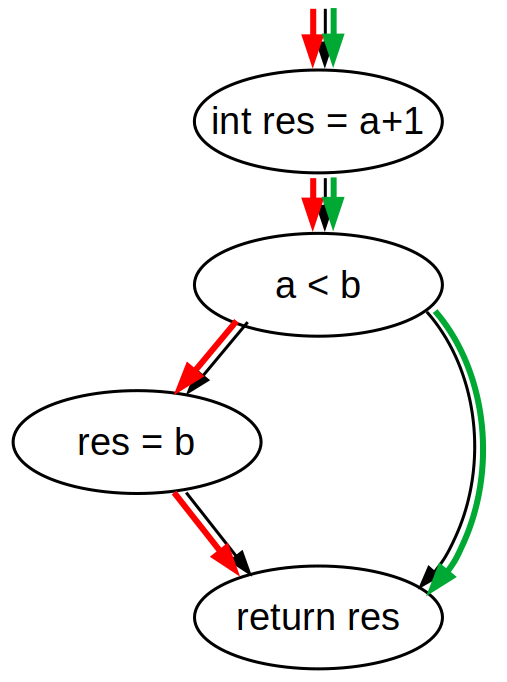
\includegraphics[scale=0.2]{Developpements/critere de test/cas_23.png}} détecte tous les arcs et donc l'erreur.

\paragraph{Critère tous les chemins} Malheurseument ce n'est pas suffisant.
\\ \\
\begin{minipage}{0.5\linewidth}
\begin{lstlisting}
max(a, b ,c):
    int res = a;
    if (res < b)
        res = b
    if (<@\sout{res} \textcolor{red}{b}@> < c)
        res = c
    return res
\end{lstlisting}
\end{minipage}
\begin{minipage}{0.5\linewidth}
\begin{center}
	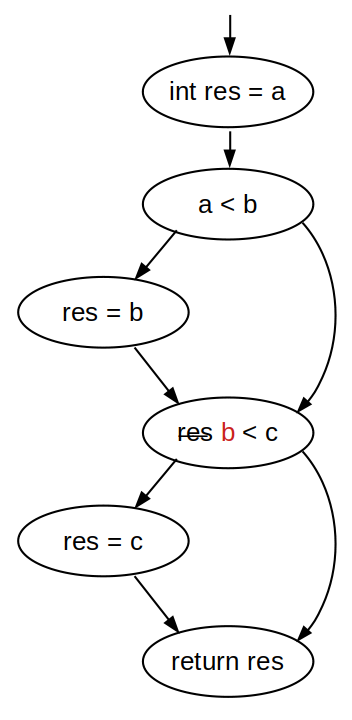
\includegraphics[scale=0.3]{Developpements/critere de test/cas_31.png}
\end{center}
\end{minipage}
\\
\begin{tabular}{c|c}
	$DT = [((3,4,5), 5), ((5,4,3), 5)]$ respecte le critère & On rajoute alors le critère tous les chemin en ajoutant \\  tous les arcs mais ne détecte pas l'erreur & $[((5,3,4), 5), ((4,5,3), 5)] $ et le premier renvoie $4$\\
	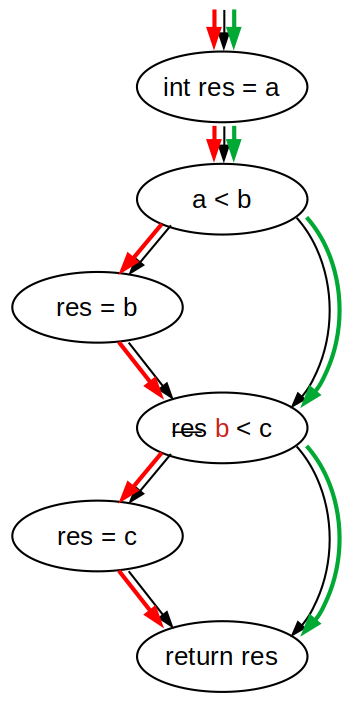
\includegraphics[scale=0.3]{Developpements/critere de test/cas_32.png} & 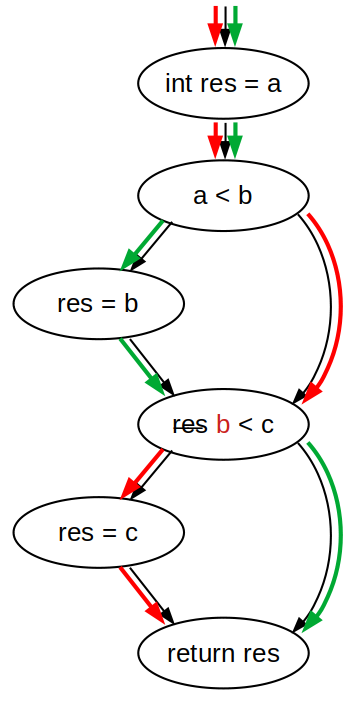
\includegraphics[scale=0.3]{Developpements/critere de test/cas_33.png}
\end{tabular}

\paragraph{Insuffisance} $DT = \big[((3,4,5), 5), \, ((5,4,3), 5), \, ((4,5,3), 5), \, ((4,3,5), 5) \big]$ Avec ca on teste tous les chemins mais on ne détecte pas le problème.

\paragraph{Insatisfiabilité} En plus de cela, les critères ne sont pas toujours satisfiables.\\
\\
\begin{minipage}{0.5\linewidth}
\begin{lstlisting}
if(true):
    res = 0
else
    res = 1
\end{lstlisting}
\end{minipage}
\begin{minipage}{0.5\linewidth}
	\begin{center}
		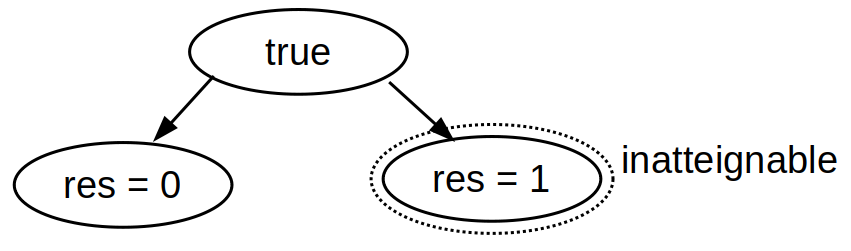
\includegraphics[scale = 0.2]{Developpements/critere de test/cas_4.png}
	\end{center}
\end{minipage}

\begin{proposition}
	Savoir si un critère est satisfiable est indécidable.
\end{proposition}
\begin{proof}
	Pour cela, on va prouver que détecter du code mort est indécidable (ce qui revient à la satisfiabilité du critère tous les noeuds, qui implique les autres).\\
	
	Procédons par l'absurde. Supposons que l'on connaisse un algorithme $\mathcal A$ qui décide si du code d'un algorithme est mort. Décidons alors le théorème de l'arrêt.\\
	
	Construisons l'algorithme $\mathcal B$ qui sur l'entrée $\mathcal C$, crée l'algorithme $\mathcal C$ puis $print(0)$. On demande alors à $\mathcal A$ si $print(0)$ est du code mort. La réponse nous dit alors si $\mathcal C$ termine ou non. Ainsi, $\mathcal B$ décide du problème de l'arrêt, pourtant indécidable.
\end{proof}

On cherche alors plutot à maximiser $\dfrac{\text{nombre d'arc visité}}{\text{nombre total d'arc}}$ (de même avec noeuds, chemins, etc...)